\documentclass[acmtog, table, dvipsnames]{acmart}
\usepackage{amsmath}
\usepackage[parfill]{parskip}
\usepackage{hyperref}

\begin{document}
\title{\textbf{Brown CS2240 Final Project Proposal} \\
       Foo}
\author{Tianmu Lan}
\author{Ruolan Tang}
\author{Kai Wang}
\begin{teaserfigure}
  \centering
  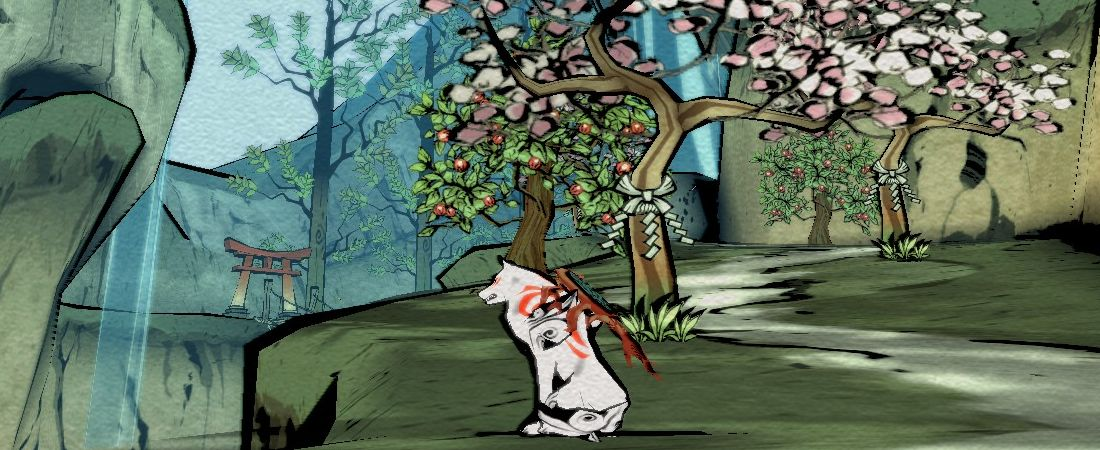
\includegraphics[width=\linewidth]{okami.jpg}
  \caption{An in game render of the game \textit{Okami} \cite{Okami}. We want to create renders with similar art styles by combining existing non-photorealistic rendering techniques.}
\end{teaserfigure}

\maketitle

\section{Introduction}

We propose to create a real-time non-photorealistic renderer with a watercolor and ink style. \textit{Okami} \cite{Okami} is a good example of a game with such a render style, though we do not aim to replicate it exactly. To achieve such an effect, two different components need to be implemented. The first component handles the watercolor-style fills, and the second component handles the pencil/ink contours. We will explore ways to handle each component, and to combine them into a stylistically coherent renderer. 
%We want to make a non-photorealistic render. When you import a 3D model or 3D scene in, you can choose to render it in watercolor style or pencil drawing style. If possible, we want to make it real-time and support some other NPR effects as well.

\section{Features}
Our current plan is to implement the features in Unity, but in general, any engine that provides easy camera control and a good support of shader programming should be suitable for our project.
\subsection{Watercolor}
The simplest way to create a watercolor effect will be a cel-shader. However, a lot of additional features can be implemented to improve the results. \cite{montesdeoca2016art} provides a good set of such features, including: 
\begin{itemize}
   \item Object-space effects, such as color bleeding technique and hand tremors effects.
   \item Watercolor reflectance model and pigment turbulence.
   \item Image-space effects, such as edge darkening, paper distortion and granulation.
\end{itemize}
We might explore addtional options as well, both from other papers and technical reports/discussions of games with similar styles.

\subsection{Pencil/Ink Contour}
Creating contours with a style of ink/pencil is a much more well studied field. There are studies that concerns how people draw those contours \cite{cole2008people}, as well as researches that concerns actual implementation \cite{praun2001real} \cite{lee2006real}. Though we have not decided upon what to do exactly, here is a list of features that we are considering:
\begin{itemize}
   \item Contour detection and contour shaking.
   \item Multiple contour drawing effects.
   \item Pencil texture generation. 
   \item Pencil texture rotation and 3-way blending.
   %\item Compositing and enhancement.
\end{itemize}
%\begin{enumerate}
%\item watercolor rendering. Shader programming. \cite{montesdeoca2016art}
%    \begin{itemize}
%	\item Controlled Object-space Effects: color bleeding technique and hand tremors effects.
%	\item Watercolor Reflectance Model and Pigment Turbulence.
%	\item Controlled Image-space Effects: Edge Darkening, Paper Distortion and Granulation.
%    \end{itemize}
%\item pencil rendering. \cite{lee2006real} \cite{praun2001real}
%    \begin{itemize}
%	\item Contour detection and contour shaking.
%	\item Multiple contour drawing effects.
%	\item Pencil texture generation. 
%	\item Pencil texture rotation and 3-way blending.
%	\item Compositing and enhancement.
%    \end{itemize}
%\end{enumerate}
%
\subsection{Extensions}
Naturally, combining methods from different works will involve a lot of occasions where we have to modify existing methods, especially if we want to create a final product that is stylistically conherent. These modification will be the major extensions that we attempt to make.

In addition, we might also try to design methods on our own, after experimenting with existing methods.
%\begin{enumerate}
%\item Try using some other methods to implement the watercolor/pencil effect.
%\item Try implementing some other stylized NPR effect on our own.
%\item Real-time rendering.
%\end{enumerate}
%
\section{Timeline}
1st week (Apr. 7th - 13th): Read relevant works and figure out mathematical details and pseudocodes for the methods we want to try out.

2nd week (Apr. 14th - 20th): Implement individual components, (likely) find more methods if previous ones don't work as intended.

3rd week (Apr 21st - 27th): Combine individual components, perform the necessary modifications to each of them.

4th week (Apr 28th - May 4th): Debug and refine the results. Make appropriate interfaces, generate results an prepare for final report and presentation.

\section{Division of Labor}
As our proposed project involves many individual components, it would be straightforward to parallelize the implementation process, as each group member can implement a selection of components. Prior to this, though, we plan to read and discuss all the methods together, to ensure that all of us have a good understanding of the entire pipeline.
%Kai Wang: Multiple contour drawing effects, Pencil texture generation. Watercolor Reflectance Model and Pigment Turbulence. Support real-time rendering.
%
%Ruolan Tang: Contour detection and contour shaking, Compositing and enhancement. Controlled Object-space Effects. UI. Try implementing other NPR effects.
%
%Tianmu Lan: Import and scene parsing. Pencil texture rotation and 3-way blending. Controlled Image-space Effects. Try implementing other NPR effects.
%
\section{Skills and Expectation}
We all have some knowledge of shader programming and relevant graphics concepts. In addition, Ruolan is familiar with Unity. We hope to develop more in depth knowledge of NPR, learn to code in the engines we choose (currently Unity), and improve our skills in reading research papers and designing complex rendering systems.
%Kai Wang:
%
%Skills: C++
%
%Predict to Acquire: more in depth knowledge about NPR
%
%Ruolan Tang: 
%
%Skills: C++ and basic graphics knowledge. PBR. Basic shader programming.
%
%Predict to acquire: more in depth knowledge about NPR. Advanced shader programming abilities. More practice on paper implementation .
%
%Tianmu Lan:
%
%Skills: C++ and basic shader implementation.
%
%Predict to acquire: more knowledge about shader implementation and more practice on paper implementation .
%
\bibliographystyle{ACM-Reference-Format}
\bibliography{main}

\end{document}

